
\chapter{Introduction}
\label{chap:Introduction} 

\section{Molecular Biology}
\label{sec:MolecularBiology}

\lettrine{M}{olecular} biology is the study of the molecular basis of biology.
It is mostly concerned with the understanding of the systems and processes
that occur within a living cell.
Naturally, the field overlaps considerably with other areas, 
such as genetics (the study of genes and heredity) and biochemistry (the study
of the chemical processes of life).

While the field itself is rather broad, much of it is underpinned by what is
referred to as the central dogma of molecular biology -- 
DNA makes RNA makes proteins.
This central dogma describes the flow of information within a cell and the
processes and control mechanisms which regulate this process.
Naturally, many of these processes are highly complicated and poorly
understood, but much progress has been made since the discovery of DNA in the
1950s to understand these processes.
Figure~\ref{fig:processes} shows the most important of these processes and how
they convert between the three most important classes of molecules in the cell.

\begin{figure}
  \centering
  \begin{tikzpicture}[node distance=5cm, auto,
      general/.style={->, >=triangle 60},
      special/.style={->, dashed, >=triangle 60}]
    \node (D) {DNA};
    \node (R) [right of=D] {RNA};
    \node (P) [right of=R] {Protein};
    \draw[general, bend left] (D) to node {\small \textit{transcription}} (R);
    \draw[general, bend left] (R) to node {\small \textit{translation}} (P);
    \draw[general] (D) to [out=110,in=70,looseness=8] 
                node {\small\textit{replication}} (D);

    \draw[special, bend left] 
      (R) to node {\small \textit{reverse transcription}} (D);
    \draw[special] (R) to [out=335,in=295,looseness=8] 
                node {\small\textit{RNA replication}} (R);
  \end{tikzpicture}
  \caption{The main processes in molecular biology. The three most common are
    shown using solid lines while two important but less common processes are
    shown in dotted lines.
    \label{fig:processes}}
\end{figure}

Molecules of DNA are the cell's long term storage mechanism -- recent research
estimates the half-life of DNA to be 521 years\cite{DNAhalflife}.
DNA molecules are long sequences of simple nucleotides which encode all the
genetic information of the cell.
Each nucleotide contains a nucleobase which is either Adenine, Guanine,
Thymine or Cytosine (A, C, G or T) and it is the sequence of so called bases 
which determines the information content of the molecule.
The nucleotides are linked together in a chain which is only read in one 
direction, known as the 5' to 3' direction.
Each base in the chain forms a hydrogen bond with a particular base from a 
complementary chain of DNA, forming a double stranded structure.
These strands are coiled around each other into DNA's characteristic 
double-helix structure.

The data stored in DNA is read by a molecule called RNA polymerase which 
produces an RNA copy of a section of the DNA in a process called
\textit{transcription}.
RNA is similar to DNA, but is short-lived (lasting minutes to hours) and so the
RNA copy is referred to as a messenger-RNA (mRNA) molecule.
This message is then read by a ribosome, a molecule which translates the mRNA 
into a protein, a process referred to as \textit{translation}.
Proteins a chain of amino acids which fold into a very specific shape and 
perform many important functions within the cell.
The region of DNA which encodes a particular protein is called a \textit{gene}.

The processes of transcription and translation through which genes are 
expressed (produce proteins) are typically very tightly
controlled by the cell, as this is the main way of influencing the levels of
various proteins within the cell and thus the cell's overall activity.

\subsection{Transcription}
\label{sec:transcription}

Both DNA and RNA have an alphabet of four symbols and so during transcription
DNA's alphabet, $\{A,C,G,T\}$, is mapped one-to-one to that
of RNA, $\{A,C,G,U\}$, where thymine is replaced with uracil.
Transcription is clearly bijective, and indeed a less common process called
reverse-transcription performs the inverse mapping from RNA to DNA.

Transcription does not act on an entire DNA strand at once but instead
transcribes a subsequence of the DNA called a transcription unit, which
contains one or many genes.
These units are marked by promoters which are regions of DNA upstream
of the transcription unit that initiate transcription by causing RNA polymerase
to bind.
They are terminated by terminator regions, which cause the RNA polymerase to
cease transcription and release the mRNA.
Modulating promoter activity in response to the concentration of another 
molecule is a common control motif.

Transcription units often contain non-coding regions called \textit{introns}
which are removed from the message in a process called RNA splicing 
before translation.
Introns do not contain any useful sequence and are often present in genes and
complicate matters significantly as efforts to predict their location 
accurately and reliably have thus far failed.

\subsection{Translation}
\label{sec:translation}

Translation is the process by which an RNA message is converted into a protein.
In higher cells (eukaryotes), mRNA undergoes further processing and is exported
from the nucleus before translation while lower organisms (prokaryotes)
translation happens as soon as possible, possibly concurrently with
transcription.

Proteins are a sequence of amino acids, where each acid comes from an alphabet
of 20 amino acids.
Each acid is coded for by 3 bases of RNA, which are referred to collectively 
as a codon.
Since there are 64 possible codons and only 20 amino acids, the code is
over complete -- several different codons map to the same amino acid.
As well as coding for amino acids, three special codons (UAG, UAA and UGA) are
known as stop codons as they terminate the translation of the protein.

In translation, molecules called ribosomes bind to the mRNA, reading the
sequence 3 bases (one codon) at a time and constructing the appropriate protein
until a stop codon is found, when the ribosome detaches and releases the
protein.

mRNA is more fragile than DNA but is also targeted by exonucleases, a class of
enzyme which degrade RNA molecules, preventing the production of more protein.
Similar processes exist to degrade proteins over time, recycling their amino
acids to form new proteins.
These degradation processes mean that a gene must continue to be transcribed at
a constant rate for the concentration of its protein to remain constant.

\subsection{Control}
\label{sec:mbio_control}

\begin{figure}
  \begin{center}
    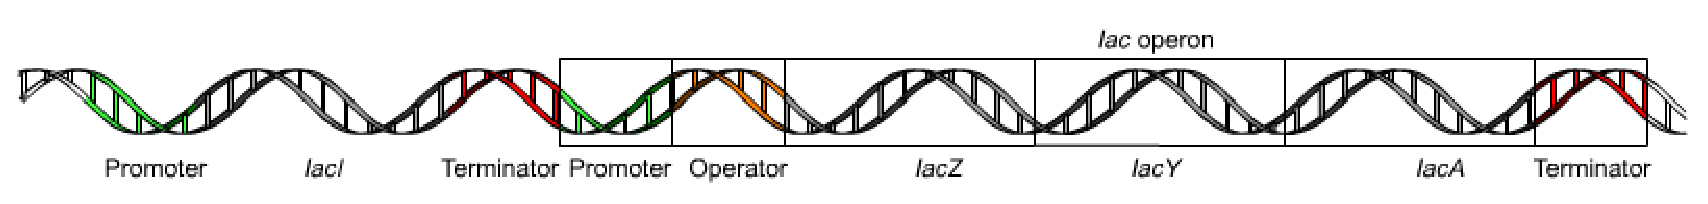
\includegraphics[width=\textwidth]{Lac_operon1}
  \end{center}
  \caption[LoF entry]{Annotated diagram of the lac operon.
    It contains two transcription units and a total of four genes.
    The first (leftmost) unit contains \textit{lacI} and is expressed 
    constitutively (continuously).
    The protein which is produced is called the lac repressor, and in the
    absence of lactose it binds tightly to the operator region, preventing
    transcription of the second transcriptional unit.
    However, when lactose is present outside the cell, a small amount will
    diffuse across the cell wall and into the cell, where it binds with the lac
    repressor, preventing it from binding to the operator and allowing
    transcription of the second unit.
    
    Of the three genes that are then expressed, two are directly relevant.
    \textit{lacY} encodes a membrane protein which actively pumps more lactose
    into the cell, causing positive feedback, and \textit{lacZ} which produces
    an enzyme which breaks down lactose into glucose and galactose which can be
    metabolised more easily.
    
    Glucose in the cell interacts with the membrane protein, reducing the rate
    at which it imports lactose and introducing a second control loop.
    As the concentration of glucose increases, less lactose is pumped into the
    cell and so the lac operon becomes less active, reducing transcription of
    the second unit.
  }
  \label{fig:lac_operon}
\end{figure}



\begin{figure}
  \centering
  \begin{tikzpicture}[auto, node distance=2cm,>=latex]
    % We start by placing the blocks
    \matrix[ampersand replacement=\&, row sep=0.15cm, column sep=0.6cm] {
      \&
      \&
      \&
      \node [block] (break) {Lactose Breakdown}; \&
      \&
    \\
      \node [input, name=glu] {}; \&
      \node [sum] (s3) {}; \&
      \node [block] (gsense) {Sensor}; \&
      \&
      \&
    \\
      \&
      \&
      \&
      \node [sum] (s2) {}; \&
      \node [branch] (br) {}; \&
      \node [output] (out) {}; 
    \\
      \node [input, name=lac] {}; \&
      \node [sum] (s1) {}; \&
      \node [block] (lsense) {Sensor}; \&
      \&
      \&
      {}; 
    \\
      \&
      \&
      \&
      \node [block] (import) {Lactose Importing}; \&
      \&
    \\};

    \node [label, right of=out, node distance=1cm] {operon\\expression};
    

    % Once the nodes are placed, connecting them is
    % easy. 
    \draw [draw,->] (glu) -- node[pos=0.01] {$[glu]$} (s3);
    \draw [->] (s3) -- (gsense);
    \draw [->] (lac) -- node[pos=0.01,swap] {$[lac]$} (s1);
    \draw [->] (s1) -- (lsense);
    \draw [->] (lsense) -| node[pos=0.95]       {$+$} (s2);
    \draw [->] (gsense) -| node[pos=0.95, swap] {$-$} (s2);
    \draw [- ] (s2) -- (br);
    \draw [->] (br) -- (out);
    \draw [->] (br) |- (import);
    \draw [->] (br) |- (break);
    \draw [->] (import) -| node[pos=0.95, swap] {$+$} (s1);
    \draw [->] (break)  -| node[pos=0.95] {$+$} (s3);

  \end{tikzpicture}
  \caption{Simplified block diagram of the lac operon, showing only the most
    important interconnections. 
    In the presence of lactose, transcription is turned on and more
    extracellular lactose is pumped into the cell, causing a positive feedback
    loop.
    Simultaneously, lactose is broken down into glucose (and galactose) which
    inhibits transcription, causing a negative feedback loop.
  }
  \label{fig:lac_block}
\end{figure}

Control of protein production is typically achieved using several layers of
control at different stages.
For example, the lac operon controls the production of enzymes which allows the
cell to metabolise lactose, a carbon source.
The cell would prefer to directly metabolise glucose if it is available as
lactose is harder to process, and so the cell can save energy by only turning
on it's lactose processing machinery when only lactose is available.
This is achieved by the lac operon as described in figure~\ref{fig:lac_operon} 
and shown schematically in figure~\ref{fig:lac_block}.

Although the lac operon was one of the first such control structures to be
discovered (and remains among the best understood), many other ingenious ways
of tightly controlling protein production have been discovered, some of which
act on transcription, some on translation and others on a combination of the
two.

\section{Synthetic Biology}
\label{sec:synbio}

Synthetic biology is a relatively new
engineering discipline with the goal of applying proven engineering techniques
such as standardisation, characterisation and encapsulation to biology.
Synbio aims to use these design principles to combine existing phenomena to 
build new, artificial forms of life.
The field is often confused with its spiritual predecessor, genetic 
engineering, which although similar in some respects does not design new
organisms, but tinkers with existing ones without trying to understand the
underlying principals.

Synbio can be thought of as programming, but with DNA instead of machine
code.
An example project which captures this idea is Tabor's bacterial edge
detector\cite{edgeDetector}.
Bacteria were programmed to produce a colourless chemical messenger in the 
absence of light and to produce a dark pigment in the presence of both light 
and the chemical messenger.
When a film of these bacteria is exposed to a pattern of light and dark, the
messenger is produced in the dark regions and diffuses into the light, where it
stimulates the production of the pigment, 
leading to an edge detection like effect.

While this and other such simple demonstrations show some of the potential 
of synbio, they lack immediate application and are of somewhat limited scope.
A major problem in expanding this work is the lack of targeted reporter
molecules.
In the edge detector example, two molecular signals are produced when light is 
not present -- AHL, a cell-to-cell signalling molecule and cI, a
transcriptional repressor molecule.
Both AHL and cI are known to affect the promoter $P_{lux-\lambda}$; while AHL 
stimulates expression, cI strongly represses it.
With expression of the dark pigment being driven by $P_{lux-\lambda}$, 
both light and AHL are required to cause the pigment to be produced.

The effect of the molecules AHL and cI on $P_{lux-\lambda}$ is one of a small
but growing number of well understood control motifs.
Since reusing the same promoter/signal combination in the same cell is 
impossible due to cross-talk, there are simply not enough signalling modalities 
available to perform more complex logic within the cell.
Indeed, it is often the case that signalling molecules have multiple functions
within the cell such that changing the concentration of one molecule to suit
our goals may cause a seemingly unrelated area of the cell's metabolism to
malfunction with undesirable consequences.

A more applicable synbio project was the effort to produce 
artemisinin (the most effective known anti-malarial) in a cheaper and more 
scalable way.
Malaria is a treatable disease which in 2010 caused roughly 2,000 deaths 
\emph{per day}, mainly because it mostly affects the developing world where
access to anti-malarials is poor.
Artemisinin is found naturally in sweet wormwood, but it is slow and expensive
to extract directly from the plant and chemical synthesis is also an expensive
and laborious process.
Synthetic biologists were able to extract the metabolic pathway responsible for
the biosynthesis of artemisinic acid (a natural precursor) and insert it into 
yeast\cite{yeast}.
Artemisinin produced in this manner has yet to be approved for sale, but it is
hoped that it should be available at some point during 2013, at a considerably
lower price than any other known method of production.

The major limiting factor in this project was yield.
In order to produce a useful amount of the drug, the metabolic pathway 
involved had to be up-regulated -- i.e. more metabolic flux directed though it.
This led to a difficult balance -- too little and very little
artemisinic acid would be produced, too high and too much of the cell's
energy would be used, causing the cells to grow slowly if at all.
As well as this, growing yeast on an industrial scale is relatively expensive.
It is desirable therefore search for host platforms which are better suited to
biosynthesis than yeast, in order to maximise the yield to cost ratio.

\section{The Chloroplast}
\label{sec:intro_plants}

Chloroplasts are a major centre for biosynthesis in plants as they perform
photosynthesis to provide energy for the plant.
The result of an ancient symbiosis, up to 1000 of these primitive cells can be 
found within each plant cell, where they make an excellent target for synbio.
They are similar to previous synbio hosts, but with access to the more
sophisticated plant cell machinery and superb potential for biosynthesis.
The native enzyme RuBisCO is so abundant in the chloroplasts that it 
can be up to 50\% of overall soluble leaf protein.

Chloroplasts contain their own DNA and expression machinery, separate from that
of the plant cell, however, they do not appear to make use of the type of
control seen in the lac operon -- instead mRNA levels appear to be
constant\cite{Sugita1996} implying that transcription in chloroplasts is always
on.
However there are clear variations in the protein levels in chloroplasts (for
example during the day/night cycle) and so control must instead be implemented 
using post-transcriptional RNA processing and/or interactions with translation.

Understanding how expression control is achieved in plant chloroplasts is a key
step in developing the potential of these organisms.
Without such an understanding, attempts to engineer synthesis pathways in them
would be reduced to genetic engineering.


